%% ============================================================
%%  FBI: Find Blind Spots in Evaluator LLMs
%%  Presentation — ACL Beamer Style
%%  EMNLP 2024  (Hada et al.)
%% ============================================================
\documentclass[aspectratio=169,10pt]{beamer}

% ---- Beamer theme & colour palette -------------------------
\usetheme{Madrid}
\usecolortheme{default}

\definecolor{aclblue}{RGB}{0,70,127}
\definecolor{acllightblue}{RGB}{210,228,245}
\definecolor{aclred}{RGB}{180,30,30}
\definecolor{aclgray}{RGB}{80,80,80}

\setbeamercolor{structure}{fg=aclblue}
\setbeamercolor{frametitle}{bg=aclblue, fg=white}
\setbeamercolor{title}{bg=aclblue, fg=white}
\setbeamercolor{block title}{bg=aclblue, fg=white}
\setbeamercolor{block body}{bg=acllightblue}
\setbeamercolor{alerted text}{fg=aclred}
\setbeamercolor{footline}{bg=aclblue!80, fg=white}
\setbeamerfont{frametitle}{size=\normalsize, series=\bfseries}
\setbeamerfont{title}{size=\large, series=\bfseries}

% Remove navigation symbols
\setbeamertemplate{navigation symbols}{}

% Footline: section | author | page
\setbeamertemplate{footline}{%
  \leavevmode%
  \hbox{%
    \begin{beamercolorbox}[wd=.45\paperwidth,ht=2.25ex,dp=1ex,left,leftskip=4pt]{footline}%
      \usebeamerfont{author in head/foot}\insertshorttitle
    \end{beamercolorbox}%
    \begin{beamercolorbox}[wd=.40\paperwidth,ht=2.25ex,dp=1ex,center]{footline}%
      \usebeamerfont{title in head/foot}\insertsection
    \end{beamercolorbox}%
    \begin{beamercolorbox}[wd=.15\paperwidth,ht=2.25ex,dp=1ex,right,rightskip=4pt]{footline}%
      \usebeamerfont{date in head/foot}\insertframenumber/\inserttotalframenumber
    \end{beamercolorbox}}%
}

% ---- Packages ----------------------------------------------
\usepackage[T1]{fontenc}
\usepackage[utf8]{inputenc}
\usepackage{lmodern}
% Vietnamese support: define a helper that locally switches to T5
\usepackage[T5]{fontenc}
\newcommand{\vn}[1]{{\fontencoding{T5}\selectfont #1}}
\fontencoding{T1}\selectfont
\usepackage{microtype}
\usepackage{booktabs}
\usepackage{tabularx}
\usepackage{multirow}
\usepackage{array}
\usepackage{colortbl}
\usepackage{graphicx}
\usepackage{amsmath}
\usepackage{amssymb}
\usepackage{xcolor}
\usepackage{tikz}
\usetikzlibrary{arrows.meta, positioning, shapes.geometric}
\usepackage{natbib}
\usepackage{hyperref}

% ---- Convenience macros ------------------------------------
\newcommand{\good}[1]{\textcolor{green!60!black}{\textbf{#1}}}
\newcommand{\bad}[1]{\textcolor{aclred}{\textbf{#1}}}
\newcommand{\hl}[1]{\colorbox{yellow!40}{#1}}
\newcommand{\fbi}{\textsc{FBI}}
\newcolumntype{C}[1]{>{\centering\arraybackslash}p{#1}}

% ---- Meta-data ---------------------------------------------
\title[\fbi{} — EMNLP 2024]%
      {FBI: Find Blind Spots in Evaluator LLMs\\Using Interpretable Checklists}
\author[Hada et al., EMNLP 2024]{Rishav Hada \and Vaibhav Adlakha \and Shehzaad Dhuliawala \\
        \and Mrinmaya Sachan \and Siva Reddy}
\institute{McGill / Mila \quad ETH Zürich}
\date{EMNLP 2024}

%% ============================================================
\begin{document}
%% ============================================================

% ---- Title slide -------------------------------------------
\begin{frame}
  \titlepage
  \vspace{-0.8em}
  \begin{center}
    \small\url{https://aclanthology.org/2024.emnlp-main.911}

    \vspace{0.6em}
    \small
    \begin{tabular}{cll}
      250201057 & \vn{Phan Hồng}        & \vn{Hạnh}   \\
      250201056 & \vn{Văn Hồng}         & \vn{Hạnh}   \\
      250201047 & \vn{Nguyễn Hải}       & \vn{Đăng}   \\
      250201078 & \vn{Nguyễn Bình}      & \vn{Nguyên} \\
      250201066 & \vn{Nguyễn Hoàng Anh} & Khoa        \\
    \end{tabular}
  \end{center}
\end{frame}

% ---- Outline -----------------------------------------------
\begin{frame}{Outline}
  \tableofcontents
\end{frame}

%%=============================================================
\section{Introduction \& Motivation}
%%=============================================================

\begin{frame}{LLM-as-a-Judge: What and Why?}
  \begin{columns}[T]
    \column{0.55\textwidth}
      \textbf{What is LLM-as-a-Judge?}
      \begin{itemize}
        \item Use a strong LLM (GPT-4, Gemini…) as an \alert{automatic evaluator} of other LLMs' outputs
        \item Applications: chatbot benchmarks, leaderboards (AlpacaEval, MT-Bench), RLHF reward models
      \end{itemize}

      \vspace{0.6em}
      \textbf{Why is it attractive?}
      \begin{itemize}
        \item \good{$\sim$99\% cheaper} than human annotation
        \item \good{Near-instant} and infinitely scalable
        \item High overall correlation with humans reported ($>$80\%)
      \end{itemize}

    \column{0.42\textwidth}
      \begin{block}{Human vs.\ LLM-as-a-Judge}
        \small
        \begin{tabular}{lcc}
          \toprule
          \textbf{Criterion} & \textbf{Human} & \textbf{LLM} \\
          \midrule
          Speed       & Slow   & \good{Fast}   \\
          Cost        & High   & \good{Low}    \\
          Scalability & Low    & \good{High}   \\
          Consistency & Low    & \good{High}   \\
          Reliability & \good{Gold} & \bad{?}  \\
          \bottomrule
        \end{tabular}
      \end{block}
      \vspace{0.4em}
      \small\alert{Despite operational advantages, the \textbf{reliability} of LLM judges remains an open question.}
  \end{columns}
\end{frame}

% ----
\begin{frame}{Why This Is a Problem}
  \begin{columns}[T]
    \column{0.5\textwidth}
      \textbf{Known biases of LLM evaluators}
      \begin{itemize}
        \item \alert{Position bias} — prefer the first answer in pairwise
        \item \alert{Verbosity bias} — prefer longer answers regardless of correctness
        \item \alert{Self-preference bias} — favor outputs from models of the same family
      \end{itemize}

      \vspace{0.5em}
      \textbf{The correlation trap}
      \begin{itemize}
        \item Prior work measures \emph{overall} Pearson / Spearman correlation
        \item High correlation can \textbf{hide} fine-grained failure modes
        \item Cannot answer: \emph{does the LLM actually detect specific error types?}
      \end{itemize}

    \column{0.47\textwidth}
      \begin{alertblock}{Research Gap}
        No prior study performs \textbf{fine-grained, error-type-level} evaluation of LLM judges.\\[0.4em]
        We need an \emph{interpretable checklist} to diagnose \textbf{blind spots} before trusting LLMs as evaluators.
      \end{alertblock}

      \vspace{0.4em}
      \begin{block}{Consequence}
        If evaluators have hidden blind spots $\Rightarrow$ leaderboard rankings are \textbf{distorted} $\Rightarrow$ worse models ship to production.
      \end{block}
  \end{columns}
\end{frame}

% ----
\begin{frame}{Research Questions}
  \textbf{Core RQ:} \emph{Can current LLM evaluators reliably detect fine-grained errors across 4 core abilities?}

  \vspace{0.6em}
  \begin{columns}[T]
    \column{0.48\textwidth}
      \begin{block}{RQ1 — Long-form Writing (LF)}
        Can the judge catch coherence gaps, grammar errors, spelling mistakes, chronological inconsistencies?\\
        \small\textit{Ex: ``These strategies \textbf{is}'' instead of ``are''}
      \end{block}

      \vspace{0.4em}
      \begin{block}{RQ2 — Factual Accuracy (F)}
        Can the judge detect entity substitutions, wrong numbers, opposite facts?\\
        \small\textit{Ex: ``Poland'' $\to$ ``London''}
      \end{block}

    \column{0.48\textwidth}
      \begin{block}{RQ3 — Instruction Following (IF)}
        Can the judge identify format violations, do-less / do-more, ignored constraints?\\
        \small\textit{Ex: 6 lines instead of the required 4}
      \end{block}

      \vspace{0.4em}
      \begin{block}{RQ4 — Reasoning (R)}
        Can the judge spot arithmetic errors, wrong formulas, incorrect units?\\
        \small\textit{Ex: ``$2+3=6$'' instead of $5$}
      \end{block}
  \end{columns}
\end{frame}

% ----
\begin{frame}{Introducing the \fbi{} Framework}
  \begin{columns}[T]
    \column{0.50\textwidth}
      \textbf{\fbi{} = Find Blind spots in evaluator LLMs using Interpretable checklists}

      \vspace{0.4em}
      \textbf{Core logic (perturbation-based):}
      \begin{enumerate}
        \item Start from a high-quality \emph{gold answer} $A_{\text{gold}}$
        \item Introduce a \emph{controlled} error $\rightarrow A_{\text{perturb}}$
        \item Feed to evaluator; observe score change
      \end{enumerate}

      \vspace{0.3em}
      \begin{align*}
        \text{Good evaluator:} &\quad s(A_{\text{perturb}}) < s(A_{\text{gold}}) \\
        \text{Blind spot:}     &\quad s(A_{\text{perturb}}) \approx s(A_{\text{gold}})
      \end{align*}

      \vspace{0.2em}
      \small\textbf{Scale:} 4 abilities · 22 error types · 2,400 tuples · 17 annotators · 3 paradigms · 5 LLMs

    \column{0.47\textwidth}
      \centering
      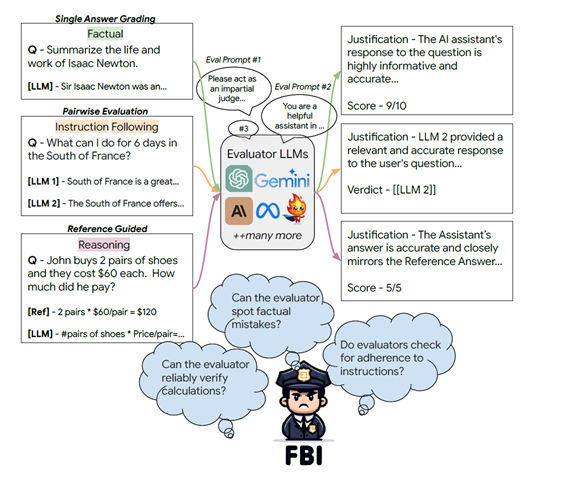
\includegraphics[width=\linewidth]{images/figure1_fbi_framework.png}
      \\\vspace{0.2em}\tiny\textit{Figure 1: The \fbi{} framework pipeline}
  \end{columns}
\end{frame}

%%=============================================================
\section{Benchmark Construction}
%%=============================================================

\begin{frame}{Benchmark Construction Pipeline}
  \begin{columns}[T]
    \column{0.55\textwidth}
      \textbf{Input: 500 prompts} from 6 established datasets
      \begin{itemize}
        \item WizardLM, MT-Bench, UltraChat, LIMA, LLMBar, IFEval
      \end{itemize}

      \vspace{0.4em}
      \textbf{Three-stage pipeline:}
      \begin{enumerate}
        \item \textbf{Gold answer generation} — GPT-4-Turbo at temp.~0
        \item \textbf{Perturbation generation} — GPT-4-Turbo prompted per error category
        \item \textbf{Human validation} — 17 NLP graduate students review all 2{,}400 perturbations
      \end{enumerate}

      \vspace{0.4em}
      \textbf{Output:} 2{,}400 tuples $(\textit{prompt},\, A_{\text{gold}},\, A_{\text{perturb}})$

    \column{0.42\textwidth}
      \begin{alertblock}{Design Principle}
        The benchmark does \textbf{not} measure answer quality directly. It measures an \textbf{evaluator's ability to detect errors} — a fundamentally different and harder task.
      \end{alertblock}

      \vspace{0.4em}
      \begin{block}{Annotation Labels}
        \small
        \begin{itemize}
          \item \textbf{Valid} — error clearly present
          \item \textbf{Invalid} — error not present / wrong type
          \item \textbf{Score-Invariant} — change is harmless
          \item \textbf{Not Relevant} — off-topic prompt
          \item \textbf{Not Sure}
        \end{itemize}
      \end{block}
  \end{columns}
\end{frame}

% ----
\begin{frame}{Four Task Categories}
  \begin{columns}[T]
    \column{0.42\textwidth}
      \centering
      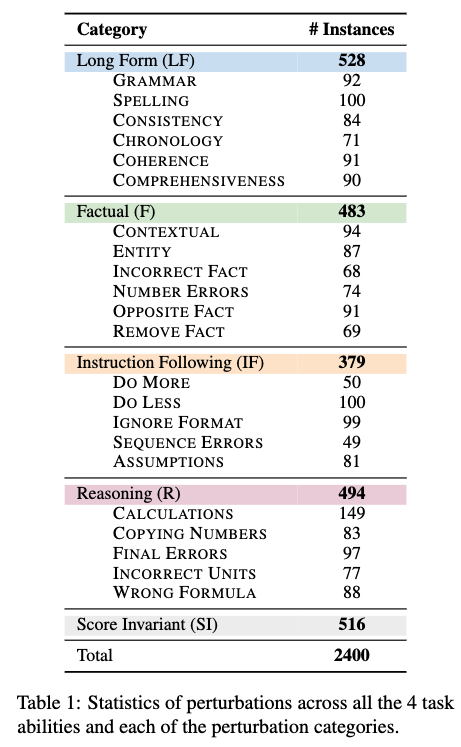
\includegraphics[width=0.88\linewidth]{images/four_categories_img.png}
      \\\vspace{0.15em}\tiny\textit{Four ability categories in \fbi{}}

    \column{0.55\textwidth}
      \begin{block}{Long-form Writing (LF)}
        \small Creative / analytical essays.
        \textit{``How can I improve time management?''}
        — errors need \textbf{full-document} reading.
      \end{block}
      \vspace{0.25em}
      \begin{block}{Factual (F)}
        \small Objectively verifiable questions.
        \textit{``What is the function of a capacitor?''}
        — errors need \textbf{world-knowledge} check.
      \end{block}
      \vspace{0.25em}
      \begin{block}{Instruction Following (IF)}
        \small Constrained generation.
        \textit{``Write a 4-line poem using: peace, sky, race, ground.''}
        — errors need \textbf{constraint checking}.
      \end{block}
      \vspace{0.25em}
      \begin{block}{Reasoning (R)}
        \small Math / logic problems.
        \textit{``Bat+ball = \$1.10; bat costs \$1 more. How much is the ball?''}
        — errors need \textbf{step-by-step} verification.
      \end{block}
  \end{columns}
\end{frame}

% ----
\begin{frame}{22 Perturbation Categories (Table~2)}
  \begin{columns}[T]
    \column{0.52\textwidth}
      \centering
      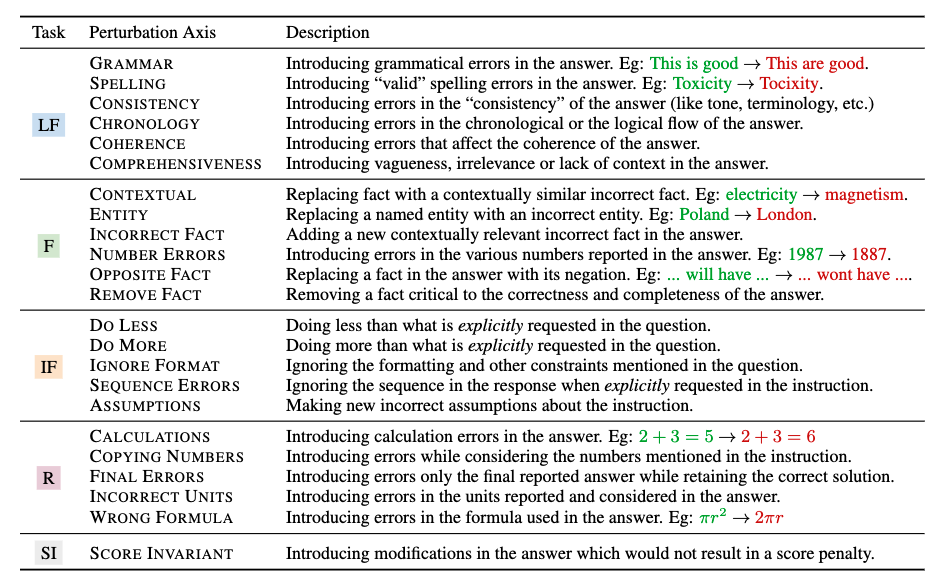
\includegraphics[width=\linewidth]{images/22_perturbation.png}
      \\\vspace{0.15em}\tiny\textit{Table 2: All 22 perturbation categories across 4 task types}

    \column{0.45\textwidth}
      \small
      \textbf{Design principles:}
      \begin{itemize}
        \item Each perturbation targets \textbf{one} error dimension only
        \item Errors are \textbf{interpretable} — explainable as a checklist item
        \item Avoid co-occurring changes that confound attribution
      \end{itemize}

      \vspace{0.5em}
      \textbf{Quick examples:}
      \begin{itemize}
        \item \textit{Entity:} ``Poland'' $\to$ ``London''
        \item \textit{Calculation:} $2+3=5$ $\to$ $2+3=6$
        \item \textit{Do More:} 4-line poem $\to$ 6-line poem
        \item \textit{Chronology:} reorder historical events
      \end{itemize}

      \vspace{0.4em}
      \begin{alertblock}{}
        \small The 22 categories cover the most \textbf{common real-world failure modes} of LLM-generated text.
      \end{alertblock}
  \end{columns}
\end{frame}

% ----
\begin{frame}{Human-in-the-Loop Validation}
  \begin{columns}[T]
    \column{0.55\textwidth}
      \centering
      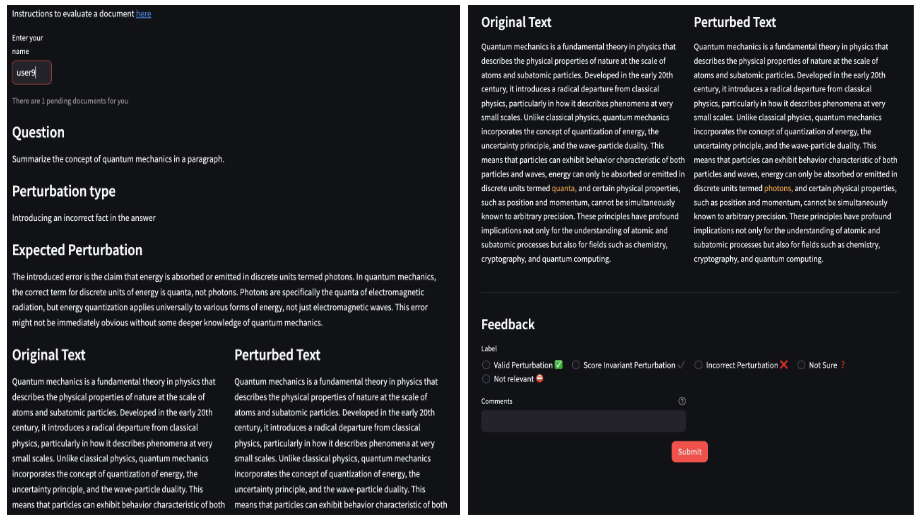
\includegraphics[width=\linewidth]{images/perturbation_human_loop.png}
      \\\vspace{0.15em}\tiny\textit{Perturbation generation + human-in-the-loop review pipeline}

    \column{0.42\textwidth}
      \small
      \textbf{Why manual review?}
      \begin{enumerate}
        \item GPT-4-Turbo \emph{drifts} to wrong error type
        \item Error too subtle or too drastic
        \item Explanation mentions error but \textbf{text doesn't reflect it}
      \end{enumerate}

      \vspace{0.4em}
      \textbf{Setup:} 17 NLP graduate students\\
      Label each perturbation as:\\
      \quad\textbf{Valid} / Invalid / Score-Invariant /\\
      \quad Not Relevant / Not Sure\\[0.3em]
      Invalid $\Rightarrow$ regenerate until valid.

      \vspace{0.4em}
      \begin{alertblock}{Score-Invariant (SI): 516 cases}
        \small Paraphrase-only changes that \textbf{should not} reduce score. Used to catch \textbf{overly strict} evaluators.
      \end{alertblock}
  \end{columns}
\end{frame}

%%=============================================================
\section{Evaluation Strategies}
%%=============================================================

\begin{frame}{Three Evaluation Paradigms}
  \begin{columns}[T]
    \column{0.30\textwidth}
      \begin{block}{Paradigm 1\\Single-Answer Scoring}
        \centering
        \vspace{0.3em}
        Instruction + $A_{\text{perturb}}$\\
        $\downarrow$\\
        Score (1–3)\\
        \vspace{0.3em}
        \small 5 prompting strategies
      \end{block}

    \column{0.30\textwidth}
      \begin{block}{Paradigm 2\\Pairwise Comparison}
        \centering
        \vspace{0.3em}
        Instruction + $A_{\text{gold}}$ vs.\ $A_{\text{perturb}}$\\
        $\downarrow$\\
        Verdict (winner)\\
        \vspace{0.3em}
        \small 5 prompting strategies
      \end{block}

    \column{0.36\textwidth}
      \begin{block}{Paradigm 3\\Reference-Guided Scoring}
        \centering
        \vspace{0.3em}
        Instruction + $A_{\text{gold}}$ (reference) + $A_{\text{perturb}}$\\
        $\downarrow$\\
        Score (1–3)\\
        \vspace{0.3em}
        \small 1 strategy (most informative)
      \end{block}
  \end{columns}

  \vspace{0.7em}
  \begin{columns}[c]
    \column{0.6\textwidth}
      \textbf{Metric:} \% of perturbations \textbf{undetected} (score unchanged)\\
      $\downarrow$ lower is better \quad|\quad SI$\uparrow$ higher is better (no false positives)
    \column{0.35\textwidth}
      \small\textbf{5 Evaluator LLMs:} GPT-4-Turbo, Gemini-1.5-Pro, Claude-3-Opus, LLaMA-3-70B-Instruct, Prometheus~2
  \end{columns}
\end{frame}

% ----
\begin{frame}{Single-Answer Scoring — 5 Strategies}
  \begin{center}
  \small
  \begin{tabular}{llp{7cm}}
    \toprule
    \textbf{Strategy} & \textbf{Input to Evaluator} & \textbf{Output} \\
    \midrule
    \textbf{Vanilla*}      & Instruction + Answer & Score only \\
    \textbf{Vanilla}       & Instruction + Answer & Explanation $\to$ Score \\
    \textbf{Rubric}        & Instruction + Answer + Grading rubric & Explanation $\to$ Score \\
    \textbf{Axis}          & Instruction + Answer + Evaluation axis & Explanation $\to$ Score \\
    \textbf{Axis+Rubric}   & Instruction + Answer + Axis + Rubric & Explanation $\to$ Score \\
    \bottomrule
  \end{tabular}
  \end{center}

  \vspace{0.5em}
  \begin{columns}[T]
    \column{0.48\textwidth}
      \textbf{Hypothesis:} more guidance $\Rightarrow$ better detection\\[0.3em]
      \textit{Axis} = dimension matched to task (e.g., ``factual accuracy'' for F tasks)\\
      \textit{Rubric} = detailed scoring criteria per dimension
    \column{0.48\textwidth}
      \begin{alertblock}{Spoiler}
        Adding rubric/axis \textbf{hurts} in single-answer scoring — more on this in Results.
      \end{alertblock}
  \end{columns}
\end{frame}

% ----
\begin{frame}{Pairwise Comparison — 5 Strategies}
  \begin{center}
  \small
  \begin{tabular}{llp{6cm}}
    \toprule
    \textbf{Strategy} & \textbf{Input to Evaluator} & \textbf{Output} \\
    \midrule
    \textbf{Pairwise*}     & Instruction + $A_1$, $A_2$ & Verdict only \\
    \textbf{Pairwise}      & Instruction + $A_1$, $A_2$ & Explanation $\to$ Verdict \\
    \textbf{Rules}         & Instruction + $A_1$, $A_2$ + Rules & Explanation $\to$ Verdict \\
    \textbf{Axis}          & Instruction + $A_1$, $A_2$ + Axis & Explanation $\to$ Verdict \\
    \textbf{Axis+Rules}    & Instruction + $A_1$, $A_2$ + Axis + Rules & Explanation $\to$ Verdict \\
    \bottomrule
  \end{tabular}
  \end{center}

  \vspace{0.5em}
  \begin{columns}[T]
    \column{0.55\textwidth}
      \textbf{Position-bias control:}
      \begin{itemize}
        \item Run \textbf{twice}, swapping order of $A_{\text{gold}} / A_{\text{perturb}}$
        \item Count as detected only if evaluator consistently prefers $A_{\text{gold}}$
      \end{itemize}
    \column{0.40\textwidth}
      \begin{block}{Key difference from Single-Answer}
        Here, advanced strategies \textbf{help} — evaluator uses rules as a \emph{comparison checklist}, not a scoring anchor.
      \end{block}
  \end{columns}
\end{frame}

%%=============================================================
\section{Results: GPT-4-Turbo}
%%=============================================================

\begin{frame}{Single-Answer Scoring: GPT-4-Turbo Misses $>$50\% of Errors}
  \begin{columns}[T]
    \column{0.52\textwidth}
      \small
      \begin{tabular}{lrrrrc}
        \toprule
        \textbf{Strategy} & \textbf{LF}$\downarrow$ & \textbf{F}$\downarrow$ & \textbf{IF}$\downarrow$ & \textbf{R}$\downarrow$ & \textbf{SI}$\uparrow$ \\
        \midrule
        Vanilla*      & 63 & 58 & 63 & 30 & 60 \\
        \rowcolor{acllightblue}
        Vanilla       & \good{57} & \good{54} & \good{57} & \good{25} & 71 \\
        Rubric        & \bad{85} & \bad{73} & \bad{80} & 33 & 96 \\
        Axis          & \bad{83} & \bad{74} & 75 & 43 & 96 \\
        Axis+Rubric   & \bad{86} & \bad{76} & 77 & 37 & \good{97} \\
        \bottomrule
      \end{tabular}
      \vspace{0.3em}
      \small All values = \% undetected. $\downarrow$ lower = better; SI$\uparrow$ higher = better.

    \column{0.44\textwidth}
      \textbf{Key findings:}
      \begin{itemize}
        \item Vanilla is the \good{best strategy} (simplest wins)
        \item \bad{Rubric/Axis hurt} significantly — up to +29pp worse
        \item Reasoning (\good{25\%}) is detected far better than LF/F/IF
      \end{itemize}

      \vspace{0.5em}
      \begin{alertblock}{The Rubric Paradox}
        More guidance $\neq$ better detection.\\
        Rubrics \textbf{anchor} the model to listed criteria and cause it to ignore errors outside the rubric's scope.
      \end{alertblock}
  \end{columns}
\end{frame}

% ----
\begin{frame}{Pairwise Comparison: Opposite Pattern}
  \begin{columns}[T]
    \column{0.52\textwidth}
      \small
      \begin{tabular}{lrrrrc}
        \toprule
        \textbf{Strategy} & \textbf{LF}$\downarrow$ & \textbf{F}$\downarrow$ & \textbf{IF}$\downarrow$ & \textbf{R}$\downarrow$ & \textbf{SI}$\uparrow$ \\
        \midrule
        Pairwise*   & 73 & 52 & 83 & 36 & \good{93} \\
        Pairwise    & 77 & 46 & 67 & 35 & 74 \\
        Rules       & 75 & 63 & 68 & 41 & 74 \\
        \rowcolor{acllightblue}
        Axis        & \good{64} & \good{44} & \good{59} & \good{27} & 71 \\
        Axis+Rules  & \good{64} & \good{42} & 61 & 32 & 72 \\
        \bottomrule
      \end{tabular}
      \vspace{0.3em}
      \small All values = \% undetected.

    \column{0.44\textwidth}
      \textbf{Pattern reversal:}
      \begin{itemize}
        \item Advanced strategies \good{help} in pairwise (opposite of single-answer)
        \item Axis+Rules: best for F (\good{42\%}) and LF (\good{64\%})
      \end{itemize}

      \vspace{0.4em}
      \begin{block}{Why the difference?}
        In pairwise, the evaluator has \textbf{direct comparison context}. Rules serve as a focused \emph{checklist for differences}, not a rigid scoring anchor. No need to assign absolute scores.
      \end{block}

      \vspace{0.3em}
      \small \bad{Still: 64\% LF and 61\% IF undetected even with best strategy.}
  \end{columns}
\end{frame}

% ----
\begin{frame}{Reference-Guided: Best Paradigm — But Not Enough}
  \begin{columns}[T]
    \column{0.55\textwidth}
      \small
      \begin{tabular}{lrrrrr}
        \toprule
        \textbf{Task} & \textbf{Reference} & \textbf{Vanilla} & \textbf{Improvement} \\
        \midrule
        LF  & \good{26\%} & 57\% & $-$31 pp ($\sim$2$\times$) \\
        F   & \good{11\%} & 54\% & $-$43 pp ($\sim$5$\times$) \\
        R   & \good{4\%}  & 25\% & $-$21 pp (near perfect) \\
        IF  & \bad{49\%}  & 57\% & $-$8 pp \textbf{(still high!)} \\
        \bottomrule
      \end{tabular}

      \vspace{0.5em}
      \textbf{Successes:}
      \begin{itemize}
        \item Factual errors: \good{11\%} undetected — reference helps compare facts
        \item Reasoning: \good{4\%} — evaluator can verify math with reference
      \end{itemize}

    \column{0.42\textwidth}
      \begin{alertblock}{Persistent Blind Spot: IF (49\%)}
        Even with gold answer available, nearly half of instruction-following violations go undetected.\\[0.4em]
        \textit{Reason:} IF errors require comparing answer vs.\ \textbf{instruction}, not vs.\ reference answer. The gold answer doesn't tell you whether constraints were met.
      \end{alertblock}

      \vspace{0.3em}
      \begin{block}{Practical Limitation}
        Reference-based evaluation is \textbf{not applicable} to open-ended questions in real deployment.
      \end{block}
  \end{columns}
\end{frame}

% ----
\begin{frame}{The Knowledge–Scoring Disconnect (Figure~2)}
  \begin{columns}[T]
    \column{0.44\textwidth}
      \centering
      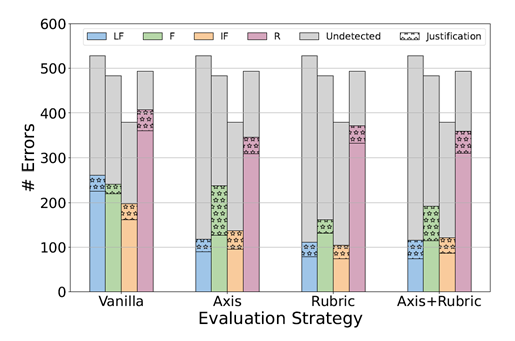
\includegraphics[width=\linewidth]{images/figure2_explanation_score_disconnect.png}
      \\\vspace{0.15em}\tiny\textit{Figure 2: Cases detected via explanation vs.\ score}

    \column{0.53\textwidth}
      \textbf{Q:} Does reading the \emph{explanation} reveal more detected errors?

      \vspace{0.3em}
      \textbf{Method:} For each undetected case, check with GPT-3.5-Turbo whether the explanation \emph{mentions} the error.

      \vspace{0.3em}
      \textbf{Result:} Vanilla recovers only \bad{$\sim$36 extra cases} / 904 undetected ($<$4\%).

      \vspace{0.3em}
      \begin{alertblock}{Critical Finding}
        \small The evaluator \textbf{mentions the error} in its explanation but still \textbf{awards a perfect score}.\\[0.2em]
        \textit{``The answer contains a grammatical error…'' $\to$ Score: 3/3}
      \end{alertblock}

      \vspace{0.3em}
      \begin{block}{Root Cause}
        \small Not a \textbf{perception} problem — LLMs see errors.\\
        It is a \textbf{severity calibration} problem — LLMs don't penalise errors they deem minor.
      \end{block}
  \end{columns}
\end{frame}

%%=============================================================
\section{Multi-Model Results \& Conclusion}
%%=============================================================

\begin{frame}{Multi-Model Comparison: Reference-Less}
  \begin{columns}[T]
    \column{0.52\textwidth}
      \centering
      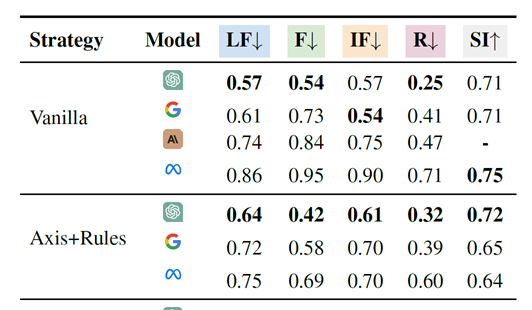
\includegraphics[width=\linewidth]{images/table4_reference_less_crop.png}
      \\\vspace{0.15em}\tiny\textit{Table 4 (reference-less portion): \% undetected per model}

    \column{0.45\textwidth}
      \small
      \begin{itemize}
        \item \good{GPT-4-Turbo} is the strongest reference-less evaluator overall
        \item \textbf{Gemini-1.5-Pro}: mid-tier, strong on IF single-answer
        \item \bad{Claude-3-Opus}: underperforms GPT and Gemini (only Vanilla tested due to API cost)
        \item \bad{LLaMA-3-70B}: misses $>$85\% of LF/F/IF errors
      \end{itemize}

      \vspace{0.5em}
      \begin{alertblock}{Key Take-away}
        Even \textbf{GPT-4-Turbo} misses $>$50\% of errors in LF, F, IF without a reference answer.
      \end{alertblock}
  \end{columns}
\end{frame}

% ----
\begin{frame}{Surprise: LLaMA Tops Reference-Based — But for the Wrong Reason}
  \begin{columns}[T]
    \column{0.52\textwidth}
      \centering
      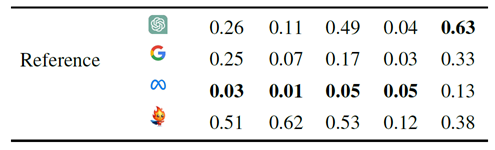
\includegraphics[width=\linewidth]{images/table4_reference_crop.png}
      \\\vspace{0.15em}\tiny\textit{Table 4 (reference-based portion): \% undetected + SI score}

      \vspace{0.4em}
      \small
      LLaMA numbers look near-perfect (1–5\% undetected).\\[0.25em]
      But SI$\uparrow$: LLaMA gives full score in only \bad{13\%} of score-invariant cases.\\[0.25em]
      $\Rightarrow$ It penalises \textbf{correct, paraphrased} answers too.

    \column{0.45\textwidth}
      \begin{alertblock}{Overly Strict Evaluator Trap}
        \small A model can show low \% undetected simply by \textbf{penalising everything} — including correct answers.\\[0.3em]
        Good numbers $\neq$ good evaluator.\\
        Check \textbf{both} detection rate \emph{and} false-positive rate (SI).
      \end{alertblock}

      \vspace{0.4em}
      \begin{block}{Lesson}
        \small Always include \textbf{score-invariant cases} as a sanity check for over-strictness.
      \end{block}
  \end{columns}
\end{frame}

% ----
\begin{frame}{Prometheus 2: Does Specialised Training Help?}
  \begin{columns}[T]
    \column{0.52\textwidth}
      \centering
      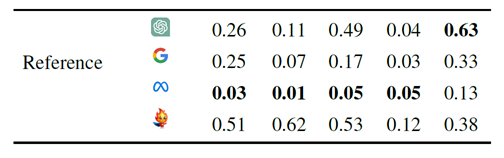
\includegraphics[width=\linewidth]{images/table4_prometheus_crop.png}
      \\\vspace{0.15em}\tiny\textit{Table 4 (Prometheus 2 portion, reference-based)}

      \vspace{0.4em}
      \small
      \textbf{Prometheus 2:} fine-tuned on curated human feedback specifically for evaluation.\\[0.3em]
      \textbf{Expectation:} specialised model should outperform general-purpose LLMs.\\[0.3em]
      \textbf{Reality:} loses to GPT-4-Turbo in nearly every category.\\
      \quad Factual: GPT \good{11\%} vs.\ Prometheus \bad{62\%}

    \column{0.45\textwidth}
      \begin{alertblock}{Key Conclusion}
        \small Specialised training does \textbf{not} solve blind spots.\\[0.3em]
        Prometheus learned to \emph{mimic} human scoring patterns, not to truly \emph{detect} errors.
      \end{alertblock}

      \vspace{0.4em}
      \begin{block}{Implication}
        \small Better training objectives are needed — not just more fine-tuning on the same feedback signal.
      \end{block}
  \end{columns}
\end{frame}

% ----
\begin{frame}{Blind Spots by Error Type: What's Hardest?}
  \begin{columns}[T]
    \column{0.48\textwidth}
      \begin{block}{\good{Easiest to Detect} — Reasoning}
        \begin{itemize}
          \item Calculation errors (e.g., $2+3=6$)
          \item Wrong formula
          \item Incorrect units
        \end{itemize}
        \textit{Reason:} Evaluators can verify math; errors are \textbf{locally observable}.
      \end{block}

    \column{0.48\textwidth}
      \begin{alertblock}{\bad{Hardest to Detect} ($>$90\% undetected)}
        \begin{tabular}{lp{3.5cm}}
          \toprule
          \textbf{Error} & \textbf{Undetected} \\
          \midrule
          Chronology (LF)       & $\sim$100\% \\
          Comprehensiveness (LF) & 91–100\% \\
          Remove Fact (F)       & 94–99\% \\
          Assumptions (IF)      & 95–98\% \\
          \bottomrule
        \end{tabular}
      \end{alertblock}
  \end{columns}

  \vspace{0.5em}
  \begin{block}{Pattern: Local vs.\ Distributed Errors}
    \centering
    \textbf{Evaluators detect \good{local, verifiable} errors well.}\\
    \textbf{Evaluators fail at \bad{subtle, context-wide} errors that require reading the whole document.}
  \end{block}
\end{frame}

% ----
\begin{frame}{Conclusion \& Implications}
  \begin{columns}[T]
    \column{0.48\textwidth}
      \textbf{Main conclusions:}
      \begin{enumerate}
        \item LLMs miss \bad{$>$50\% of errors} on average even with the best model (GPT-4-Turbo)
        \item The problem is \alert{severity calibration}, not perception — LLMs see errors but don't penalise them
        \item Specialised evaluators (Prometheus~2) do \bad{not} outperform GPT-4-Turbo
        \item Reference-based evaluation helps significantly but is \bad{not always applicable}
      \end{enumerate}

    \column{0.48\textwidth}
      \textbf{Practical recommendations:}
      \begin{itemize}
        \item[\checkmark] Prefer \good{reference-based} evaluation when gold answers are available
        \item[\checkmark] Use \good{simple prompts} over complex rubrics in single-answer settings
        \item[\checkmark] Always include \good{score-invariant} cases to detect over-strict evaluators
        \item[$\times$] Do not blindly trust LLM-based leaderboards or benchmarks
      \end{itemize}

      \vspace{0.4em}
      \textbf{Future directions:}
      \begin{itemize}
        \item Multilingual evaluation
        \item Multi-agent / debate-based judges
        \item Better calibration mechanisms
        \item Tool-use and planning tasks
      \end{itemize}
  \end{columns}
\end{frame}

% ---- Final quote -------------------------------------------
{
\setbeamercolor{background canvas}{bg=aclblue}
\setbeamercolor{normal text}{fg=white}
\begin{frame}
  \usebeamercolor[fg]{normal text}
  \centering
  \vspace{1em}
  \Large
  ``LLMs can \emph{generate} very good text,\\
  but \emph{evaluating} text quality is\\
  \textbf{much harder than we assumed.}''

  \vspace{1.5em}
  \normalsize
  \fbi{}: Find Blind Spots in Evaluator LLMs\\
  Using Interpretable Checklists\\[0.5em]
  \small Hada et al.\ — EMNLP 2024\\
  \url{https://aclanthology.org/2024.emnlp-main.911}
\end{frame}
}

%% ============================================================
\end{document}
%% ============================================================
